\documentclass{article}
\title{ChucK Assignment 5}
\date{10 May 2012}
\usepackage{fullpage}
\usepackage{listings}
\usepackage{url}
\usepackage{graphicx}
\usepackage{textcomp}

\begin{document}
\maketitle

\textsl{This lesson will discuss using arrays to create pitch collections, concurrency with Machine.add(), and recording to disk.}\vspace{2mm}

You've learned much of what ChucK is capable of at the audio level. Now we're going to focus on some techniques to create polyphony (multiple notes at once), recording your ChucK output to an audio file. But first we're goint to talk about arrays.

\section{Arrays}

\begin{itemize}

\item Arrays are variables made up of \textbf{ordered lists.} That is, an array allows you to store a list of numbers and access them in order.

\item Think of a row of mailboxes for an apartment building. All of the boxes are at the same address, but they have different apartment numbers.

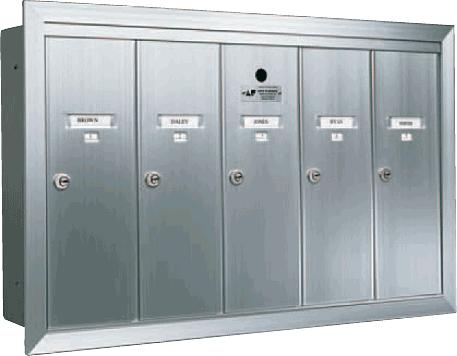
\includegraphics[scale=0.3]{apt_boxes}

An array is a variable, so it has a type (like int, float, or dur), a name, and a size (the number of ``boxes''):

\begin{lstlisting}
 int myApartmentBldg[5]; // creates an array with 5 elements
 83 => myApartmentBldg[0]; // sets the first element of the array to 83
 24 => myApartmentBldg[1]; // sets second element to 24
\end{lstlisting}

\item One of the most common uses of an array is to create a collection of pitches. Take careful note of how this code is laid out:

\begin{lstlisting}
 [60, 62, 64, 67, 69] @=> int pentatonic[];
\end{lstlisting}

There's a new operator above: @=\textgreater, called the \textsl{assignment operator.} This is a special case where you can't use the usual =\textgreater to set something.
\pagebreak
\item Now that we've created our pentatonic scale, we need to access it. Like so many computer-related things, we start counting from 0, so the first item in the array is \textbf{pentatonic[0]}, the second is \textbf{pentatonic[1]}, and so on.

\begin{lstlisting}
TubeBell m => dac;
pentatonic[0] => m.freq;
1 => m.noteOn;
1::second => now;
pentatonic[1] => m.freq;
1 => m.noteOn;
1::second => now;
\end{lstlisting}

\item Heads up! The first element in the array is [0]. That means the \textbf{last} item is [size-1]. So if you make an array
\textbf{int num[5]} and try to use num[5] you'll get an ArrayOutOfBounds error. You will make this error. We all do, and often.

\item Before we go on, identify the error in each of these four code examples, and suggest how to fix it.

\begin {enumerate}
\item Find the error:

\begin{lstlisting}
int badArray[10];
0.5 => badArray[0]; // ERROR!
\end{lstlisting}

\item Find the error:

\begin{lstlisting}
dur timings[10];
5::second => timings; // ERROR!
\end{lstlisting}

\item Find the error:

\begin{lstlisting}
[0.8, 0.3, 0.1] => float mallets[]; //ERROR!
\end{lstlisting}

\item Find the error:

\begin{lstlisting}
float pan[12];
0.46 => pan[12]; // ERROR!
\end{lstlisting}

\end {enumerate}

\item \textbf{Arrays} and \textbf{for} loops are a classic combination. The 
\textbf{for} loop cycles through the array, retrieving values.
The following code is a very typical way to use an array.

\begin{lstlisting}
// REICH MELODY
ModalBar mb => dac;
[64, 66, 71, 73, 74, 66, 64, 73, 71, 66, 74, 73] @=> int pianoPhase[];
for (int i; i<12; i++) // loop from 0 to 11
{
 pianoPhase[i] => Std.mtof => mb.freq; // convert to freq and assign to mb
 1 => mb.noteOn; // start note
 150::ms => now; // pass time
}
\end{lstlisting}

\section {Concurrency}

\item I have intentionally held off on introducing \textsl{concurrency,} the ability to
do multiple sounds at once, but I know you're eager to create more complex textures. There are a couple of methods of concurrency, but we're going to start with the simplest. You already know that you can run multiple ``shreds" at once in the virtual machine. Well, you can tell your code to do that too.

\item You're going to start with a ChucK script that makes sound. Open one of our earlier assignments, or go to the Course Documents page on Blackboard and download concurrency1.ck and concurrency2.ck. \textbf{Save them in your home folder, or move them there after you've saved them.}

\item Now open a new blank ChucK file in the miniAudicle. Enter the code below and save it in your home folder.

\begin{lstlisting}
Machine.add("concurrency1.ck"); // change the name in quotes if
				// you're using your own ChucK file
5::second => now;
Machine.add("concurrency2.ck");
\end{lstlisting}

\item Now hit the ``add" button and watch as it launches the two files.

\section {Recording to audio file}

So you want to share your ChucK sounds with others? This requires a new object called \textbf{WvOut}, as well as the strange new world of the \textbf{blackhole}!

\item Open one of your earlier ChucK scripts (not one that runs forever). Add this to the top of your code:

\begin{lstlisting}
 dac => WvOut mySound => blackhole;
 "prettysounds" => mySound.wavFilename;
\end{lstlisting}

Hmm... OK, it makes sense that if WvOut records, it should get input from the dac. But what the heck is the blackhole??

Synthesizing audio takes up processor power. The more things running at once, the greater the demands on your computer. But ChucK reduces that as much as it can. You see, if you create this:
\begin{lstlisting}
 SinOsc s;
\end{lstlisting}
ChucK recognizes that it's not connected to the output, so it doesn't even calculate it! We say that \textsl{the dac reaches back,} meaning it activates the UGens that output into it.

But you don't want to send the output of WvOut into the dac; you just want it to be activated. That's what the blackhole is for. It's a silent sample calculator. The blackhole activates UGens like the dac does, but it doesn't pass the UGen's audio to the output.

\item Now, at the end of your code, add this to close out the audio file:

\begin{lstlisting}
 mySound.closeFile();
\end{lstlisting}

And that's it! Save and run your file and a new audio file will be created in the same directory as your script.

\end{itemize}

\textbf{Assignment 3: Piano Phase}\vspace{2mm}
\\
\textbf{Create a version of Steve Reich's Piano Phase using the REICH MELODY code from page 2. Record 1 minute of it using WvFile and upload the audio file to Blackboard by Tuesday, May 15 at 11:59 pm. Feel free to mess around with the melody or timbre, but don't destroy the essential phasing character of the piece.}
\pagebreak
\center{ \textbf{Tips for realizing Reich's Piano Phase with ChucK}}\vspace{2mm}
\\
\begin{enumerate}
\item You'll need 3 ChucK files, all saved in your home directory. Two of them contain \textsl{nearly identical} code (based on the REICH MELODY code from page 2) while the other has the Machine.add() functions.
\item In order for the phasing to occur, you'll need to alter how quickly time passes between notes for one of the REICH MELODY scripts.
\item The REICH MELODY code only plays through the array once. You'll need to create a loop to make it repeat. Put the ``main'' section of the code in a while(true) loop to make it repeat forever.
\item Since each of the phasing instruments has a gain of 1, when they're both playing the total gain is 2. This will result in unpleasant digital distortion. Reduce the gains of the ModalBar instruments so they don't exceed 1.
\item The WvOut object will be placed in the same file as Machine.add(). At the end of that file, you will advance time by 1 minute (1::minute =\textgreater now;). Don't forget to tell ChucK to close the audio file.
\end{enumerate}
\end{document}
